\chapter*{Úvod}
\addcontentsline{toc}{chapter}{Úvod}
Už v antike sa niektorý antický folozofi zaoberali myšlienkou, že základ jendotlivých druhov sa časom mení.
A práve v gréčtine môžme nájsť pôvod slova \emph{Fylogenéza}, kde fylé = kmeň a genesis = zrodenie/pôvod.
Fylogenéza sa zaoberá vývojom druhu organizmov, väčšinov sa odohráva počas príliš dlhého časového úseku, 
preto ju niesme schopný priamo pozorovať a nezostáva nám iná možnosť ako vytvoriť rekonštrukciu na základe evolučných poznatkov.
Neskôr v tomto vednom poli urobil významný pokrok Charles Darwin keď v roku 1859 publikoval svoju knihu \emph{Pôvod druhov},
okrem toho, že z evolúcie vytvoril široko uznávanú teóriu, predstavil aj myšlienku spoločného predka, kedy akékoľvek dva veľmi rozdielne
druhy zdieľajú spoločného prapredka a vizuálne ju znázornil vo forme stromového grafu, takzvaného \emph{stromu života}.
Tak položil základy Evolučnej histórie, ktorá skúma evolučné procesy, ktoré
na zemi vytvorili rôznorodosť života z počiatočnej živej formy. 
Dalšie poznatky v oblasti genetiky, súvisejúce s DNA a RNA viedli k tomu, že na evolúciu sa
dodnes pozeráme hlavne prostredníctvom génov.
Sekvenovanie DNA umožinilo vzťahy medzi jednotlivými organizmami odsledovať na základe zmien ktoré prebehli v ich DNA sekvencie.
To nám ponúka množstvo presných dát využitelných pri rekonštrukcii fylogenetického procesu.
Aj na našej fakulte vzniklo niekoľko prác, ktoré sa venujú rekonštrukcii DNA sekvencie pokiaľ poznáme jej súčasný vzhľad,
prípadne sa snažia zrekonštruovať fylogenetický strom pokiaľ poznáme DNA sekvencie súčasných druhov.
\cite{Kovac2011,Hozza2014,Herencsar2014,Vinar2010}. 
\begin{figure}[t]
 \centering
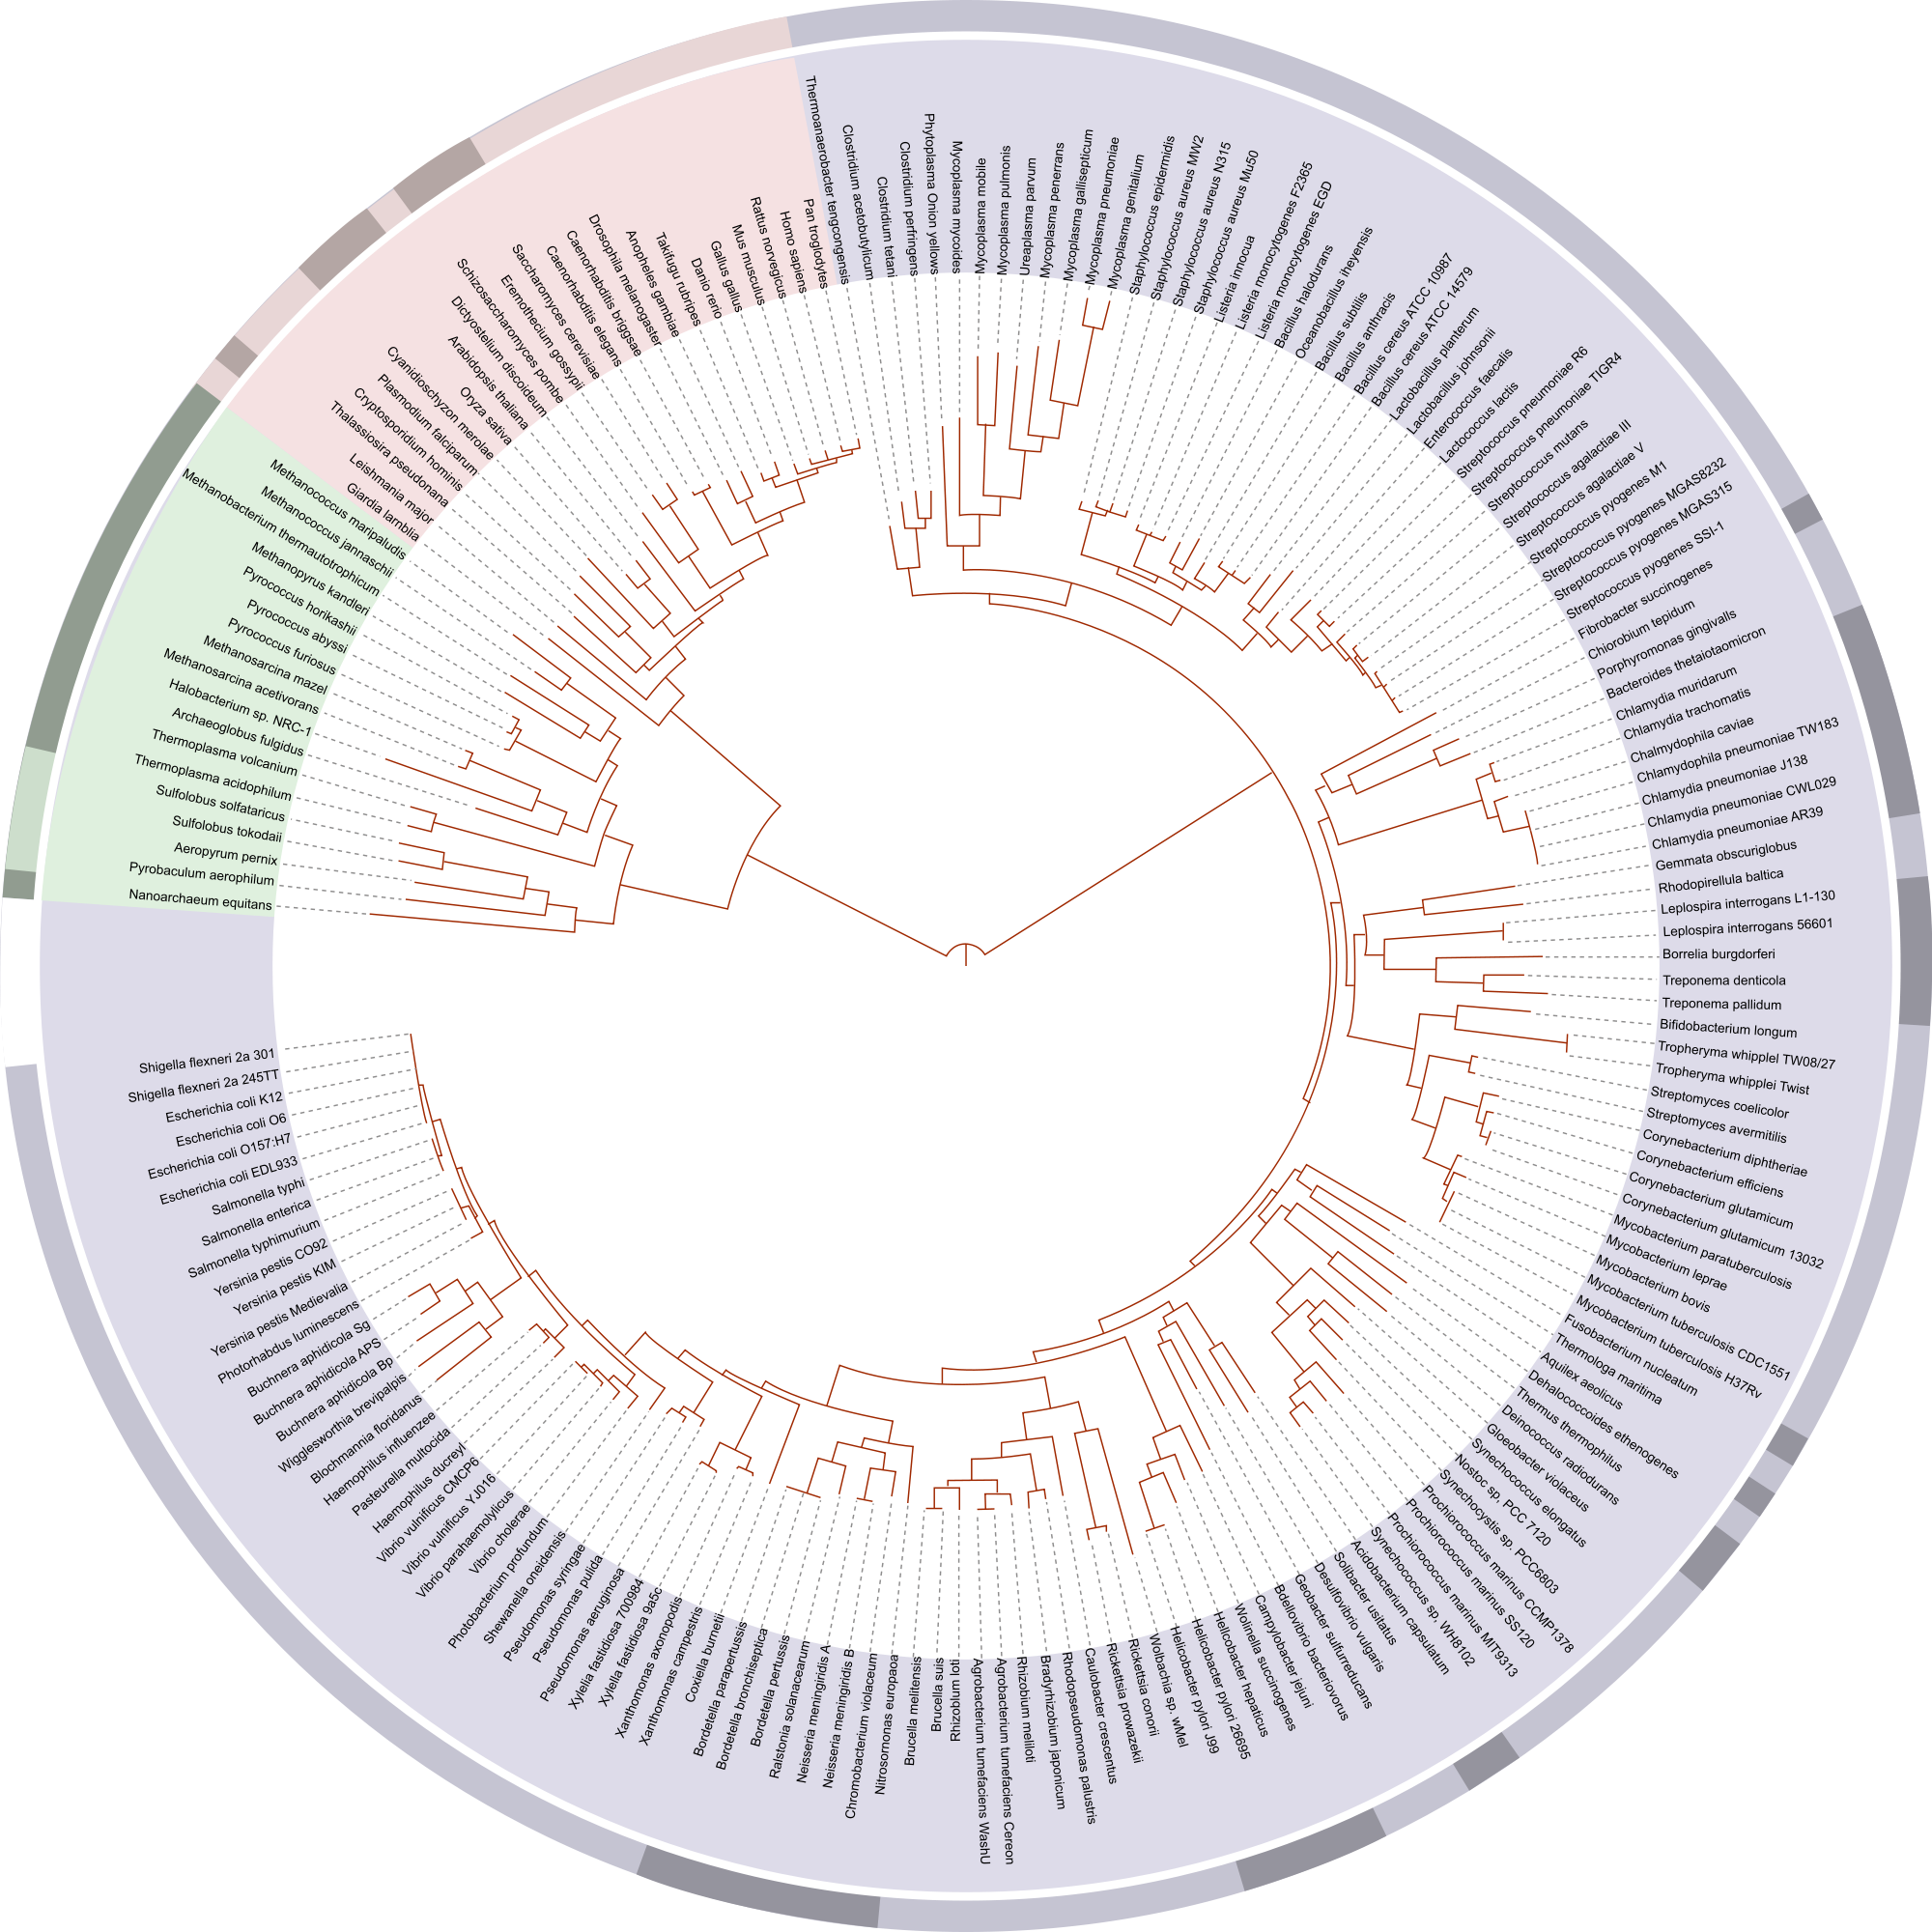
\includegraphics[width=1\textwidth]{images/tol}
\caption{Strom života, Zdroj: wikipedia.org}\label{obr:tol}
\end{figure}

Strom stále patrí medzi najpopulárnejšie spôsoby ako zobraziť evolučné vzťahy medzi druhmi alebo inými objektami.
Najčastejšie sa stretávame so stromom života, kedy je snaha zobraziť vývoj druhov z posledného spoločného prapredka, ako napríklad vidíme na obrázku \ref{obr:tol}.
V týchto prípadoch sa samotné zmeny DNA do zobrazenia nezvyknú dostať, informácie ktoré nám poskytnú, 
ako napríklad vzdialenosť dvoch objektov na základe rozdielnosti ich DNA sekvencie, však bývajú použité na zostavenie takéhoto zobrazenia.
Cieľom tejto práce je zostrojiť program ktorý nám zobrazí jednoduchú postupnosť sekvencí DNA s dôrazom na zmeny ktoré sa udiali s génmy v týchto sekvenciách.
Výsledok by mal predstavovať malú vetvu fylogenetického stromu v ktorom prepojenie objektov zobrazí reálne zmeny ktoré sa odohrali na ich DNA sekvencii.
Inšpiráciou pre túto prácu sú vyššie spomenuté práce pochádzajúce z našej fakulty,
náš program má byť schopný vizualizovať výsledky ktoré produkujú a poslúžiť okrem iného ako rýchla optická kontrola správnosti.

Prvá kapitola nám poskytne úvod do problemtaiky, predstavíme si základné pojmy potrebné pre našu prácu.

Druhá kapitola sa bude venovať implementácii nášeho programu, pozrieme sa na to ako vyzerá jeho vstup a výstup,
aké možnosti interakcie poskytuje uživateľovi a ktoré nastavenia v ňom vieme meniť.

Tretia kapitola nám povie prečo chceme zobraziť iba niektoré gény a akým spôsobom ich budeme vyberať.

Štvrtá kapitola nadväzuje na tretiu, porovnávame v nej aké výsledky dostaneme v závislosti od toho, aký spôsob výberu génov zvolíme.
